\documentclass[twocolumn,aps,pre,amsmath,amssymb,floatfix,longbibliography]{revtex4-1}
\usepackage{graphicx}
\usepackage{dcolumn}
\usepackage{bm}
\usepackage{amsfonts}
\usepackage{xcolor,tabu}
\usepackage{multirow}
\usepackage{amsthm}
\usepackage{tikz}
\usepackage[colorlinks=true,
            linkcolor=blue,
            urlcolor=blue,
            citecolor=blue]{hyperref}
\hypersetup{bookmarksopen=true}


\begin{document}

\title{Correlations and Giant Number Fluctuations in 3-D Bacterial Suspenions}

\author{Zhengyang Liu}
%\email{liux3141@umn.edu}
\author{Wei Zeng}
\author{Xiaolei Ma}
\author{Xiang Cheng}


\affiliation{Department of Chemical Engineering and Materials Science, University of Minnesota, Minneapolis, Minnesota 55455, USA}

\date{\today}

\begin{abstract}
Active systems, such as bacterial suspensions, exhibit strong spatial correlations and giant number fluctuations, which are known as signatures of such systems. Models have predicted how concentration and dimension affect correlations and number fluctuations, but real progress is still limited by lacking of experimental data. Here, we present a quantitative study on correlations and density fluctuations at various concentrations in 3 dimensional space. Giant number fluctuations get stronger as the concentration is increased, which reaches a plateau when concentration is above the turbulence transition. In particular, we observe a nontrivial fluctuation below the turbulence transition, indicating that pushers such as \textit{E. coli} swim in a correlated way. Our kinetics study reveals the underlying mechanisms of giant number fluctuations.
\end{abstract}

\maketitle
\section{Introduction}

Bacterial suspensions are premier example of active matter. Being constantly driven out of equilibrium, they exhibit anomalous properties drastically different from systems in equilibium, including enhanced diffusivity, reduced viscosity and giant number fluctuations. While the anomalous diffusion and rheology have only been demonstrated in microscopic scale, the giant number fluctuations are predicted to be more universal across various length scales. Indeed, such fluctuations have been observed in bird flocks \cite{Ballerini1232}, fish schools \cite{Ward6948}, shaking granules \cite{Narayan105}, bacteria on agar gels \cite{Zhang13626} and active actin filaments \cite{Schaller4488}.

Despite the extensive efforts to measure giant number fluctuations in a variety of systems, a few limitations remain to be overcome. First, although it is intuitive that the number fluctuation at high concentration (ordered state) is much stronger than that at low concentration (disordered state) \cite{PhysRevE.95.020601, Zhang13626}, the effects of concentration can be more complicated than binary. All experiments so far have oversimplified the concentration effects and a detailed measurement in need. Second, the kinetics (or growth) of giant number fluctuations has been overlooked. The kinetics itself can reveal an intrinsic time scale of an active system. More importantly, comparisons can be made with kinetics of other quantities \cite{Peng2020}, such as flow order and flow energy, to reveal the underlying mechanisms of giant number fluctuations. Third, while theories predict an explicit dependence on dimensionality \cite{doi:10.1146/annurev-conmatphys-031119-050752}, all simulations and experiments have been in 2-dimensional spaces. A measurement in 3-D is needed to test the theories.

% few measurements on 3-D systems are reported due to the difficulty in directly counting particle numbers in microscopic 3-D systems. From theoretical point of view, the 3-D measurements of giant number fluctuations are of key importance since the scaling of number fluctuations is predicted to be dependent on dimensionality [1]. This missing piece motivates us to investigate the giant number fluctuations in 3-D systems.

Most \textit{E. coli} strains use oxygen as their primary energy source. In a closed chamber, they deplete oxygen quickly and the motility decreases markedly. To overcome this limitation, we use a light-controlled \textit{E. coli} strain, whose primary energy source is light, so that the swimming speed can be instantaneously and precisely controlled. Without oxygen depletion issue, the concentration effects can be investigated in closed samples. In addition to solving the oxygen depletion issue, the light-controlled \textit{E. coli} strain allows us to study the kinetics of giant number fluctuations. Existing experiments have always been in 2-D, due to the difficulty in directly counting particle numbers in a 2-D image of a 3-D sample, where images of many layers superpose. Inspired by earlier experimental works, where image intensity was used to indicate local number density \cite{PhysRevLett.106.018101, Schaller4488}, we overcome the challenge of directly counting particle` numbers and are able to use image intensity variations to quantify the number fluctuations in a 3-D bacterial suspension.


Here, we show that \textit{E. coli} suspensions at concentrations above 60 n$_0$ shows giant number fluctuations with $\Delta N \varpropto N^\alpha$, where $\alpha\approx0.83$, close to the predictions on dry active nematics (0.83) and dry active polar fluids(0.76). Remarkably, the scaling exponent, $\alpha$, shows a dependence on concentration below 60 n$_0$, which does not vanish at 20 n$_0$ (below the active turbulence transition, 40 n$_0$). This nontrivial dependence on concentrations below the active turbulence transition suggests that giant number fluctuations can arise without apparent collective motion (where groups much larger than individuals moving together can be identified), in consistency with a recent theoretical work \cite{PhysRevLett.119.028005}.

% This fluctuation is shown to result from topological defects in the associate flow field, where transient high density "clusters" appear and disappear.

%\begin{figure}[!]
%\begin{center}
%\includegraphics[]{}
%\caption[]{}
%\end{center}
%\end{figure}

\section{Experiment}

\subsection{Light-controlled bacteria}
We introduce a light-driven transmembrane proton pump, proteorhodopsin (PR), to wild-type \textit{E. coli} (BW25113) by transforming the bacteria with plasmid pZE-PR encoding the SAR86 $\gamma$-proteobacterial PR-variant \cite{Walter2408}. The activity of PR is directly correlated with the light intensity. Thus, we can control the swimming speed of bacteria using light of different intensities.

The bacteria are cultured at 37 \textcelsius with a shaking speed at 250 rpm for 14-16 hours in terrific broth (TB) [tryptone 1.2\% (w/w), yeast extract 2.4\% (w/w), and glycerol 0.4\% (w/w)] supplemented with 0.1 g/L ampicillin. The culture is then diluted 1: 100 (v: v) in fresh TB and grown at 30 \textcelsius for 6.5 hours. PR expression is triggered by supplementing the culture medium with 1 mM isopropyl $\beta$-D-thiogalactoside and 10 \textmu M ethanolic all-trans-retinal in the mid-log phase (3 hours after the dilution).

The bacteria are harvested by gentle centrifugation (800g for 5 min). After discarding the culture medium in the supernatant, we resuspend bacteria with dI water. The resuspended suspension is then centrifuged again at 500g for 5 min, and finally adjusted to target concentration for microscopy.

\begin{figure}[!]
\begin{center}
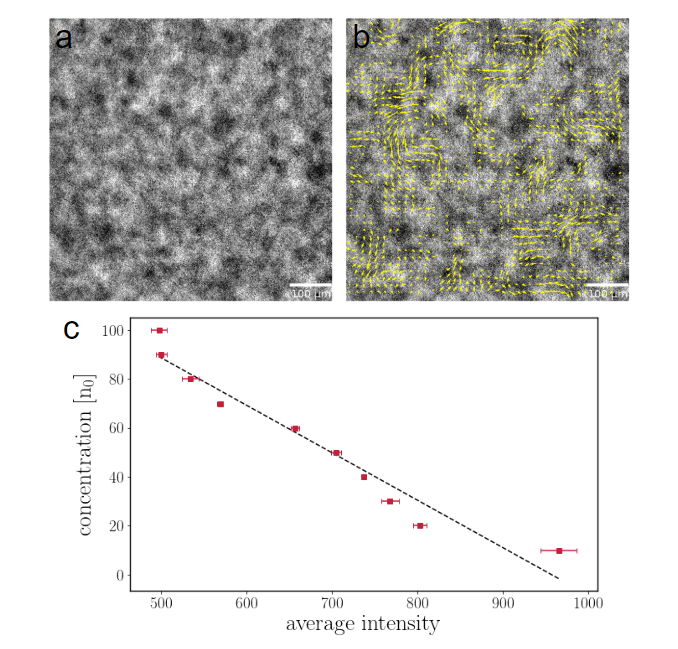
\includegraphics[width=0.45\textwidth]{GNF-figures-1.png}
\caption[]{Bright-field microscopy of a bacterial suspension at 80 n$_0$ (a) and the velocity field at the instance (b). Scale bar is 100 \textmu m. (c) Relation between bacterial suspension concentrations (measured by OD600 spectrometer) and average image intensities (red squares). Error bars represent the standard deviations of pixel intensities in an image. The black dashed line is a linear fitting of the relation. }
\label{fig:1}
\end{center}
\end{figure}

\subsection{Sample preparation and microscopy}

To prepare the sample for microscopy, we put bacterial suspensions prepared from the previous step into a seal chamber made of glass slides (25 mm $\times$ 75 mm) and coverslips (18 mm $\times$ 18 mm). We first glue (Norland 81) two coverslips on a glass slide, side-by-side, leaving a 3-mm separation between the two coverslips. We then cover the 3-mm separation with another coverslip to form a "channel". Then we use pipet to inject bacterial suspensions into the channel. Finally, we seal the two ends of the channel using UV glue (Norland 76) to form a sealed chamber.

The sample bacterial suspensions are images through an inverted bright-field microscope using a 20$\times$ (NA 0.5) objective. The filed of view is 640 $\times$ 640 \textmu m$^2$ (Fig.~\ref{fig:1}a). In order to control the velocity of bacteria by light, we wait for 10 minutes after loading samples so that bacteria can deplete the disolving oxygen in the samples and stop swimming when light is switched off. Then we switch on the light to trigger the light-powered motility. We wait another 2 minutes for the collective motion to reach a steady state under the new light condition, and start to take images. All the videos are recorded at 30 frames per second using a sCMOS camera.

\subsection{Kinetics}
The growth of giant number fluctuations is imaged when we tune up the swimming speed of \textit{E. coli} by light. Videos are taken at 30 FPS for 1 minute. The light intensity is tuned from low to high at 5 seconds. Note that, to avoid a short unstable period of the light source when adjusting the voltage (\textcolor{red}{SI figure unstable\_light}), we set the voltage fixed at high at the beginning of each experiment. In the first 5 seconds, the light source is blocked with a neutral density filter, which is then removed to achieve high light intensity.

\subsection{Correlation analysis}

\subsubsection{Flow fields}
The flow fields are measured by Particle Image Velocimetry (PIV) analysis using openPIV package in Python \cite{openpiv} (Fig.~\ref{fig:1}b). We choose box size to be 16 \textmu m, which is much larger than a single bacterium body to enhance statistical accuracy, and smaller than the typical length scale of the collective motion of \textit{E. coli} so that the features are not smoothed out. We choose step size to be half of the box size (8 \textmu m) by convention.

\subsubsection{Concentration fields}
The concentration fields are measured directly from the image pixel intensity fields. In an attempt to calibrate the concentration-intensity relation, I fix the light intensity on microscope, and load bacterial samples of various concentrations. Then I plot the concentrations as a function of corresponding average image pixel intensities, as shown in Fig.~\ref{fig:1}c. This result suggests that concentration and image intensity follows approximately a linear relation, or formally:
$$ c = aI + b $$
where $c$ is bacterial concentration, $I$ is pixel intensity, $a$ and $b$ are constants. This linear relation will be used in the number fluctuation calculation in Sec.~\ref{sec:method_gnf}.
\subsubsection{Spatial correlations}

The spatial correlation of a quantity $A$ (concentration, velocity or orientation) is defined as the following:

$$ C(x, y) = \frac{\langle(A(x_0+x, y_0+y)-\bar A)(A(x_0, y_0)-\bar A) \rangle_{x_0, y_0}}{\langle(A(x_0, y_0)-\bar A)^2\rangle_{x_0, y_0}}$$

where $\langle\cdot\rangle_{x_0, y_0}$ denotes the spatial average of a quantity over all possible $x_0$'s and $y_0$'s.  $\bar A$ denotes the spatial average of $A$, i.e. $\bar A=\langle A\rangle_{x_0, y_0}$.

\subsubsection{Temporal correlations}
The temporal correlation of a quantity $B$ (concentration) is defined as the following:

$$ C(\tau) = \frac{\langle (B(t+\tau)-\bar B)(B(t)-\bar B)\rangle_t}{\langle(B(t)-\bar B)^2\rangle_t} $$

where $\langle\cdot\rangle_{t}$ denotes the spatial average of a quantity over all possible $t$'s.  $\bar B$ denotes the temporal average of $B$, i.e. $\bar B=\langle B\rangle_{t}$.

\subsubsection{Coarse-graining}
All the correlation analyses are done on coarse-grained data. On the one hand, we obtain velocity fields using PIV, which requires the image to be divided into interrogation boxes. On the other hand, the pixel size of our image is 0.33 \textmu m, which is much smaller than a \textit{E. coli} bacterium. As a result, the intensity of a single pixel may reflect the local concentrations of a suspension, but rather the structures within one bacterium body. Therefore, we divide our images into boxes of the same size as is used in PIV analysis, for the concentration field correlation analysis (and the giant number fluctuation analysis).

As discussed above, the box size needs to be larger than the size of a \textit{E. coli} bacterium. In addition, it should not be larger than the correlation length of the concentration or velocity fields, so that the correlations can still be captured after coarse-graining. We varied the box size and step size to perform PIV analysis, and it turns out that setting box size at 16 \textmu m and step size at 8 \textmu m gives reasonable results (SI figure \textcolor{red}{step\_choice}).

\subsection{Giant number fluctuation analysis}\label{sec:method_gnf}
Two methods have been used to quantify giant number fluctuations. One of them, which divides a frame of an image sequence into small boxes and measure the standard deviation of particle numbers in these boxes. Then the procedure is repeated over all the frames, and the average of the standard deviations gives a measure of number fluctuations of the system (Menon 2007). The other method, which also divides images into small boxes, measures the standard deviations of numbers of particles in each box over time. Then the standard deviations are averaged in space to give a measure of number fluctuations of the system (Urbach 2008). Urbach 2008 futher stated that when a system is homogeneous, where spatial and temporal correlations are small compared with the system size and experiment duration, two methods give the same result. Our experimental system, \textit{E. coli} suspensions, has a correlation length ($\sim 50$ \textmu m) much smaller than the system size ($\sim 170$ \textmu m, or 1 cm), and is thus a spatially homogeneous system. However, since we rely on image pixel intensity to indicate the local concentrations, a slight inhomogeneity of illumination would result in a long standing concentration inhomogeneity, which is not true in reality (see SI figure \textcolor{red}{inhomogeneity}).

Therefore, we use the second method, since the illumination inhomogeneity is long standing and stable over time. We can think of it as adding a constant image to each frame, which does not affect the temporal variation calculation. We take box size ranging from 10 to 30 \textmu m, and examine the temporal variations of bacterial concentrations $\Delta N_{ij}$ in the $i^{th}$ box for each box size $l_j$. The temporal variations are then averaged in space (over $i$) to give a single value variation $\Delta N_{j}$. Then number fluctuations in the system is captured by the dependence of $\Delta N_{j}$ on $l_j$. In an equilibrium system, $\Delta N_{j}\propto l_j$ (this follows from $\Delta N_{j}\propto \sqrt{N_j}$ and $N_j\propto l_j^2$). Thus, the deviation from $\Delta N_{j}\propto l_j$ quantifies the giant number fluctuation in the system. Here, we plot $\Delta N_{j}/l_j$ as a function of $l_j^2/l_b^2$. To be consistent with the notations in literatures, we get rid of the subscript $j$, and write $l_j$ as $\sqrt{N}$. We still note here that the subscript $j$ indicates different choices of box sizes.

\section{Results and discussion}

\begin{figure}[!]
\begin{center}
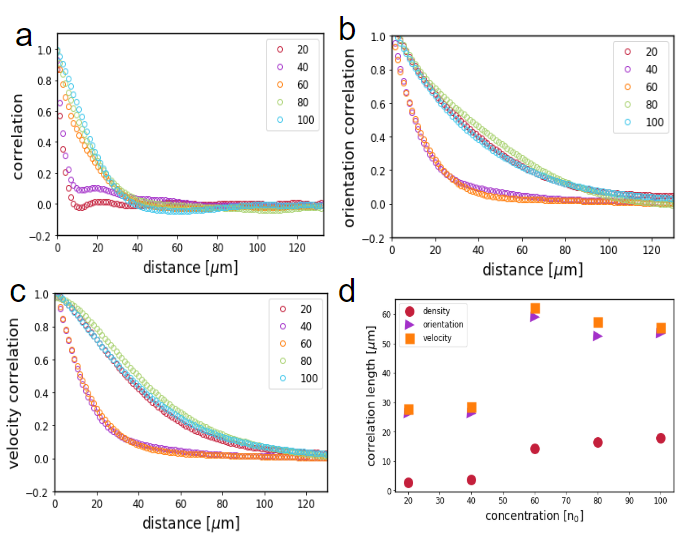
\includegraphics[width=0.5\textwidth]{GNF-figures-2.png}
\caption[]{(a) Spatial correlation of image intensity (b) Spatial correlation of flow orientation (c) Spatial correlation of velocity (d) Correlation length (defined as $C=1/e$) of intensity, orientation and velocity at concentrations = 20, 40, 60, 80 and 100 n$_0$.}
\label{fig:2}
\end{center}
\end{figure}

\begin{figure}[!]
\begin{center}
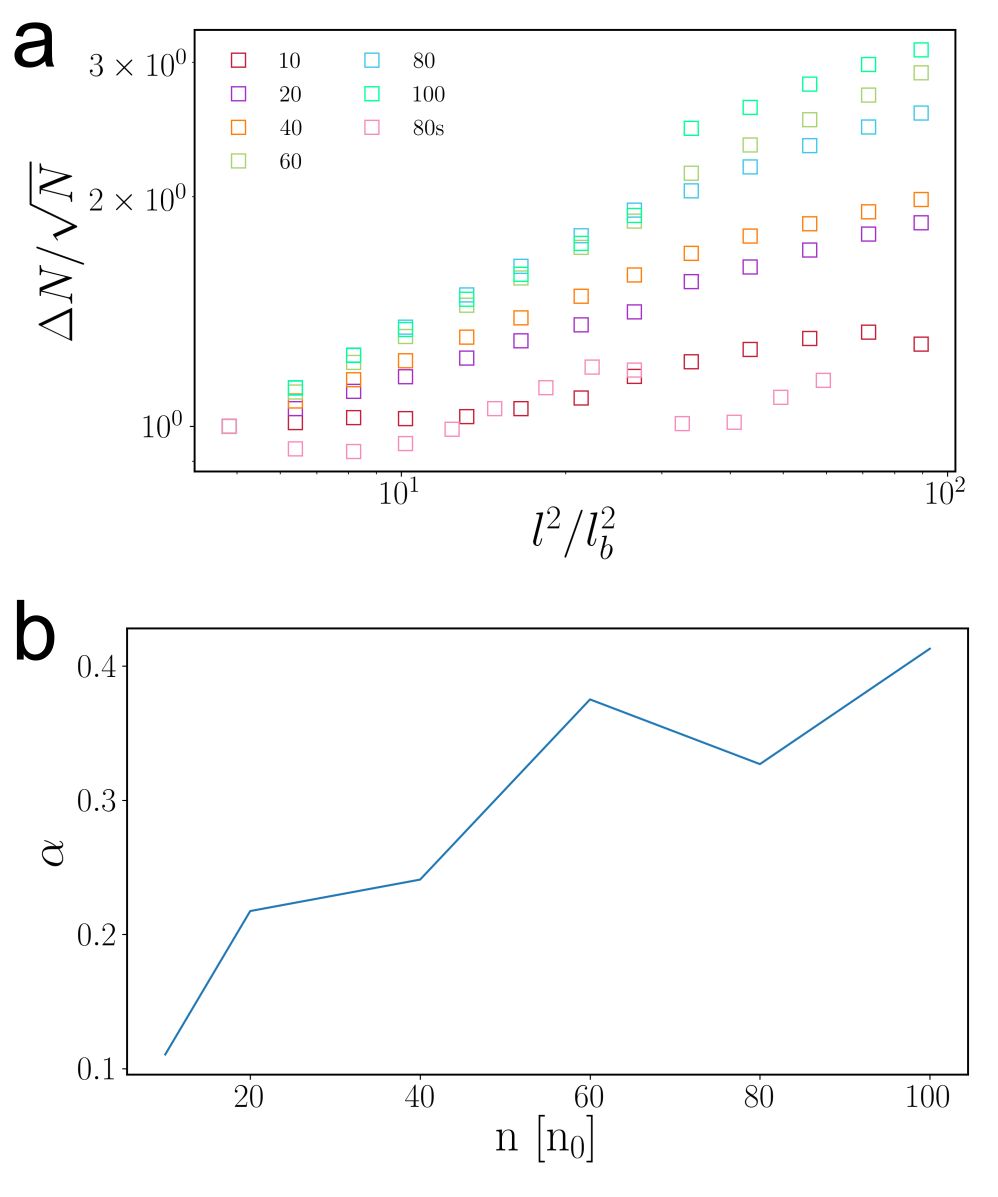
\includegraphics[width=0.5\textwidth]{GNF-figures-3.png}
\caption[]{(a) Giant number fluctuations in bacterial suspensions at concentrations = 10, 20, 40, 60, 80, 100 n$_0$. The $\Delta N/\sqrt{N}$ is in fact $\Delta I/l$, where $I$ is the average pixel intensity of a subsystem and $l$ is size of the subsystem. The $\Delta I/l^2$ value is rescaled by the first value of each curve, so that all the curves start from $\Delta I/l=1$. The 80s (pink) curve shows the number fluctuations of a static (velocity=0) sample. (b) The scaling exponents $\alpha$ ($\Delta N \propto N^{0.5+\alpha}$) of number fluctuation curves as a function of bacterial concentrations. }
\label{fig:3}
\end{center}
\end{figure}

\begin{figure}[!]
\begin{center}
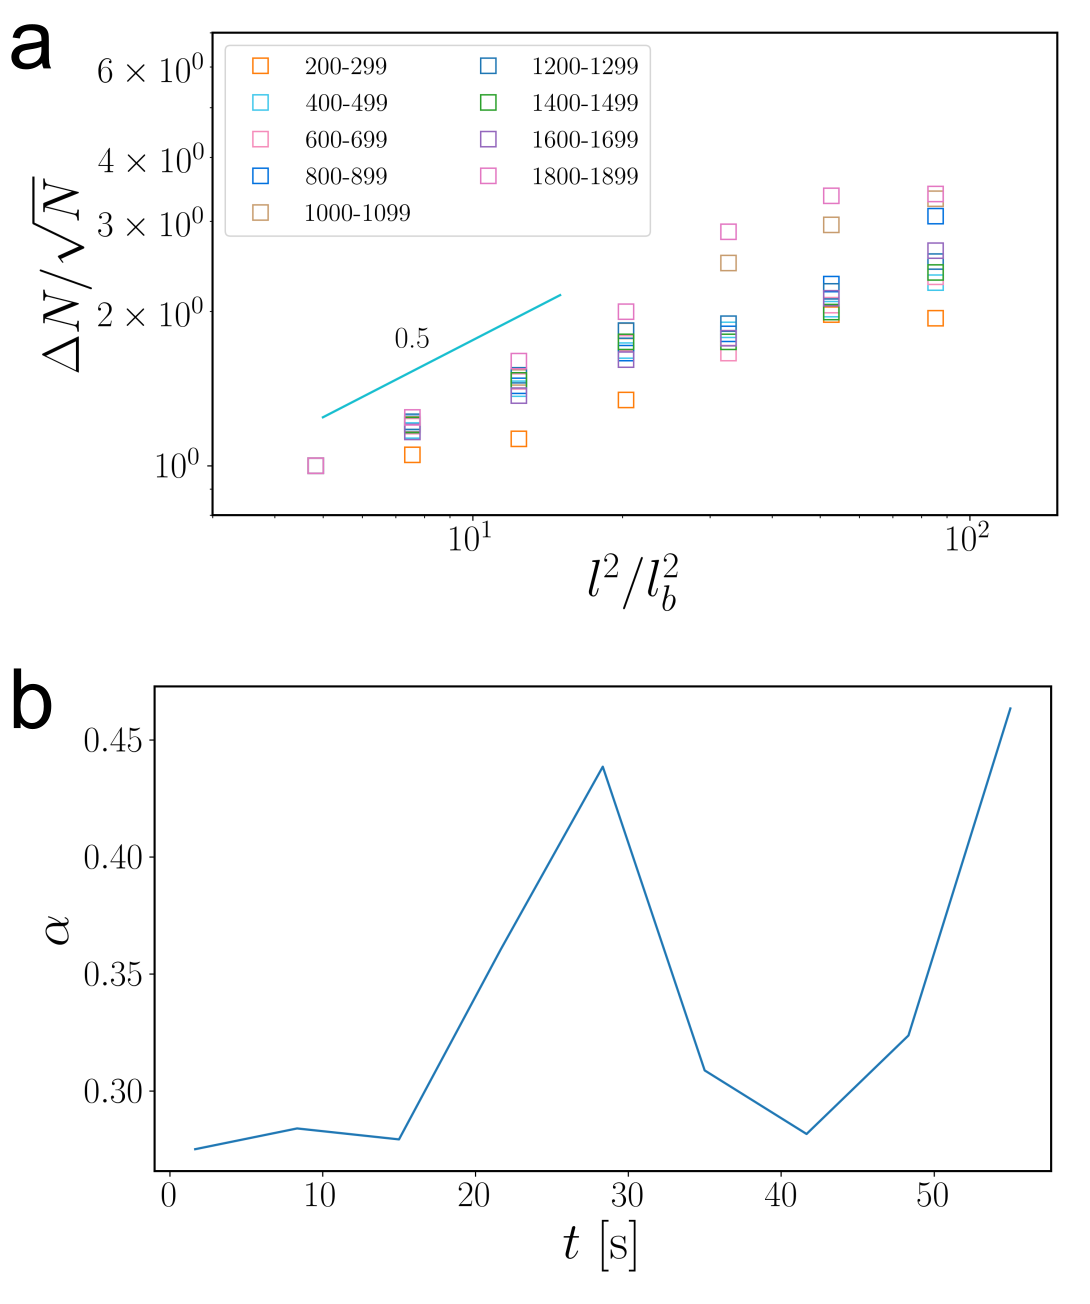
\includegraphics[width=0.5\textwidth]{GNF_kinetics_conbine.png}
\caption[]{Evolution of giant number fluctuations at concentration $n=100$ n$_0$. (a) Number fluctuations rescaled by the square root of average particle number $\Delta N/\sqrt N$ as a function of subsystem size rescaled by bacterial body size $l^2/l_b^2$. Numbers in legends marks the time (frame, videos are taken at 30 frames per second).  (b) The scaling exponents $\alpha$ ($\Delta N \propto N^{0.5+\alpha}$) of number fluctuation curves as a function of time.}
\label{fig:4}
\end{center}
\end{figure}

\begin{itemize}
\item Correlation Results
\item GNF Result
\item interplay Results
\item discussion (wave, lifetime, length scale implication, low concentration correlation, etc)
\end{itemize}

\subsection{Spatial correlations}
We analyzed the spatial correlations of concentration, flow orientation and flow velocity (Fig.~\ref{fig:2}a-c) of motile \textit{E. coli} suspensions at various concentrations. All the correlation lengths increase dramatically as we increase the concentration from 40 n$_0$ to 60 n$_0$. The crossover suggests a transition from a disordered state to ordered or collective state. Remarkably, we show that the correlation length of concentration exhibit the crossover at the same concentration as those of flow orientation and flow velocity (Fig.~\ref{fig:2}d). (\textcolor{red}{Need to make sure if this is the first report on using concentration correlation to mark turbulence transition.}) While the spatial correlations of flow orientation and flow velocity have been used in earlier works, no one has reported on using concentration (or image pixel intensity) correlation to quantitatively determine turbulence transition. This consistency makes it more convincing to use image pixel intensity as an indicator of local bacterial concentration.

\subsection{Giant number fluctuations}
Giant number fluctuations are observed in our experiments.

\subsubsection{Varying concentration}
 We show that bacterial suspensions at different concentrations exhibit giant number fluctuations to different degrees (Fig.~\ref{fig:3}a). In particular, unlike a sudden crossover observed in the correlation lengths, we observe a gradual increase of scaling exponent $\alpha$ when increasing concentration $n$ (Fig.~\ref{fig:3}b). \textcolor{red}{Say more about the fluctuations below turbulence transition.}

\subsubsection{Kinetics}
We also study the kinetics of giant number fluctuations. By virtue of the light-controlled \textit{E. coli}, we are able to image how a "dead" suspension gradually start to mix, form patterns, and deviate from the central limit theorem. Fig.~\ref{fig:4}a shows the number fluctuations at 100 n$_0$. Fig.~\ref{fig:4}b shows how the scaling exponent changes over time.

\textcolor{red}{Most importantly, this study unveils the underlying mechanism of giant number fluctuations when compared with the evolution of other quantities (order parameter and flow energy).}
\section{Conclusions}
We find something

\section*{Acknowledgments}

\bibliographystyle{apsrev4-2}
%\bibliography{cracks}
\bibliography{correlations}



\end{document}
